	%%%
	%%% V7
	%%%

	\subsection{Polymorphismus in Haskell} % (fold)
	\label{sub:polymorphismus_in_haskell}
		\begin{itemize}
			\item parametrischen über Typvariablen
			\item ad-hoc übr Typklassen
		\end{itemize}

		\subsubsection*{Unterschied} % (fold)
		\label{ssub:unterschied}
			\begin{tabular}{lcp{8cm}}
				ad-hoc & $\equiv$ & derselbe Name für unterschiedliche Algorithmen\\
				parametrischer & $\equiv$ & derselbe Name für den gleichen Algorithmus, also ein Algorithmus für alle Typen
			\end{tabular}
		% subsubsection unterschied (end)

		\subsubsection*{Beispiel parametrischer Polymorphismus} % (fold)
		\label{ssub:beispiel_parametrischer_polymorphismus}
			\lstHaskell
			\begin{lstlisting}
length :: [a] -> Int
length [] = 0
length (_:l) = 1 + length l
			\end{lstlisting}
		% subsubsection beispiel_parametrischer_polymorphismus (end)
	% subsection polymorphismus_in_haskell (end)

	\subsection{Weltveränderung} % (fold)
	\label{sub:weltveraenderung}
		\lstHaskell
		\begin{lstlisting}[morekeywords={sgetLine}]
sgetLine :: IO String
		\end{lstlisting}
		\lstHaskell
		\begin{lstlisting}
p :: IO a
q :: IO b
p >> q :: IO b
p >> q = \w -> let (a,w') = p w
                   (b,w'') = q w'
               in (b,w'')
		\end{lstlisting}
		Was nichts anderes ist als
		\lstHaskell
		\begin{lstlisting}
p >> q = q.snd.p
		\end{lstlisting}
		\lstHaskell
		\begin{lstlisting}
getChar :: IO Char
putChar :: Char -> IO ()
		\end{lstlisting}
		\lstHaskell
		\begin{lstlisting}
(>>=) :: IO a -> (a -> IO b) -> IO b
p :: IO a
f :: a -> IO a

p >>= f :: IO b
p >>= f = \w -> let (a,w') = p w
                    (b,w'') = w'
                in (b,w'')
		\end{lstlisting}
		\lstHaskell
		\begin{lstlisting}
do {a; b} == do a
                b
		\end{lstlisting}
		\lstHaskell
		\begin{lstlisting}
{f;g;}h; != f;{g;h;}
		\end{lstlisting}
		\lstHaskell
		\begin{lstlisting}
data Ampel = Rot
           | Gelb
           | Gruen
data Tree a = Nil |
              Node a Tree Tree
		\end{lstlisting}
		\lstHaskell
		\begin{lstlisting}[mathescape]
IO (\w -> ((),w)) $\equiv$ IO \$ \w -> ((),w)
		\end{lstlisting}

		%%%
		%%% end V7
		%%%
		%%%
		%%% V8
		%%%

		\lstHaskell
		\begin{lstlisting}
-- generisch
MState s a

-- konkret
MS (\x -> (x,17))

-- und damit Typ
MState s Int
		\end{lstlisting}

		\lstHaskell
		\begin{lstlisting}
bla = MS (\x -> (x,17))
(runMState bla) :: s -> (s,Int)
		\end{lstlisting}

		\lstHaskell[Mitzählen von \texttt{getc} als Aktion, aber keine Auslieferung]
		\begin{lstlisting}
getc = \s -> (s+1,s)
		\end{lstlisting}

		\lstHaskell[Zähler zurücksetzen]
		\begin{lstlisting}
put = \s' -> MS $ \s -> (s',s)
		\end{lstlisting}

		\lstHaskell[Kurzform vereinfacht Nutzung und Schachtelung]
		\begin{lstlisting}
-- Langform
MState s a

-- Kurzform
m a

-- Nutzung
instance Monad m where
		\end{lstlisting}

		\lstHaskell[detaillierte Aufschlüsselung anhand von \texttt{get >>= put}]
		\begin{lstlisting}
get = MS (\s -> (s,s))
put = \s' -> MS (\s -> (s',s))
runMState (MS f) = f

get >>= put

MS (\s -> let (s',a) = runMState (MS (\s -> (s,s))) s
          in runMState (put s) s')
MS (\s -> let (s',a) = (\s -> (s,s)) s
          in runMState (put s) s')
MS (\s -> let (s',a) = (s,s)
          in runMState (put s) s')
MS (\s -> runMState (put s) s)
MS (\s -> runMState (MS (\s -> (s,s))) s)
MS (\s -> (\s -> (s,s)) s)
MS (\s -> (s,s))
		\end{lstlisting}
		
		\begin{figure}[ht]
			\caption{Realisierung Verkettung äußerer mit innerer Monade}
			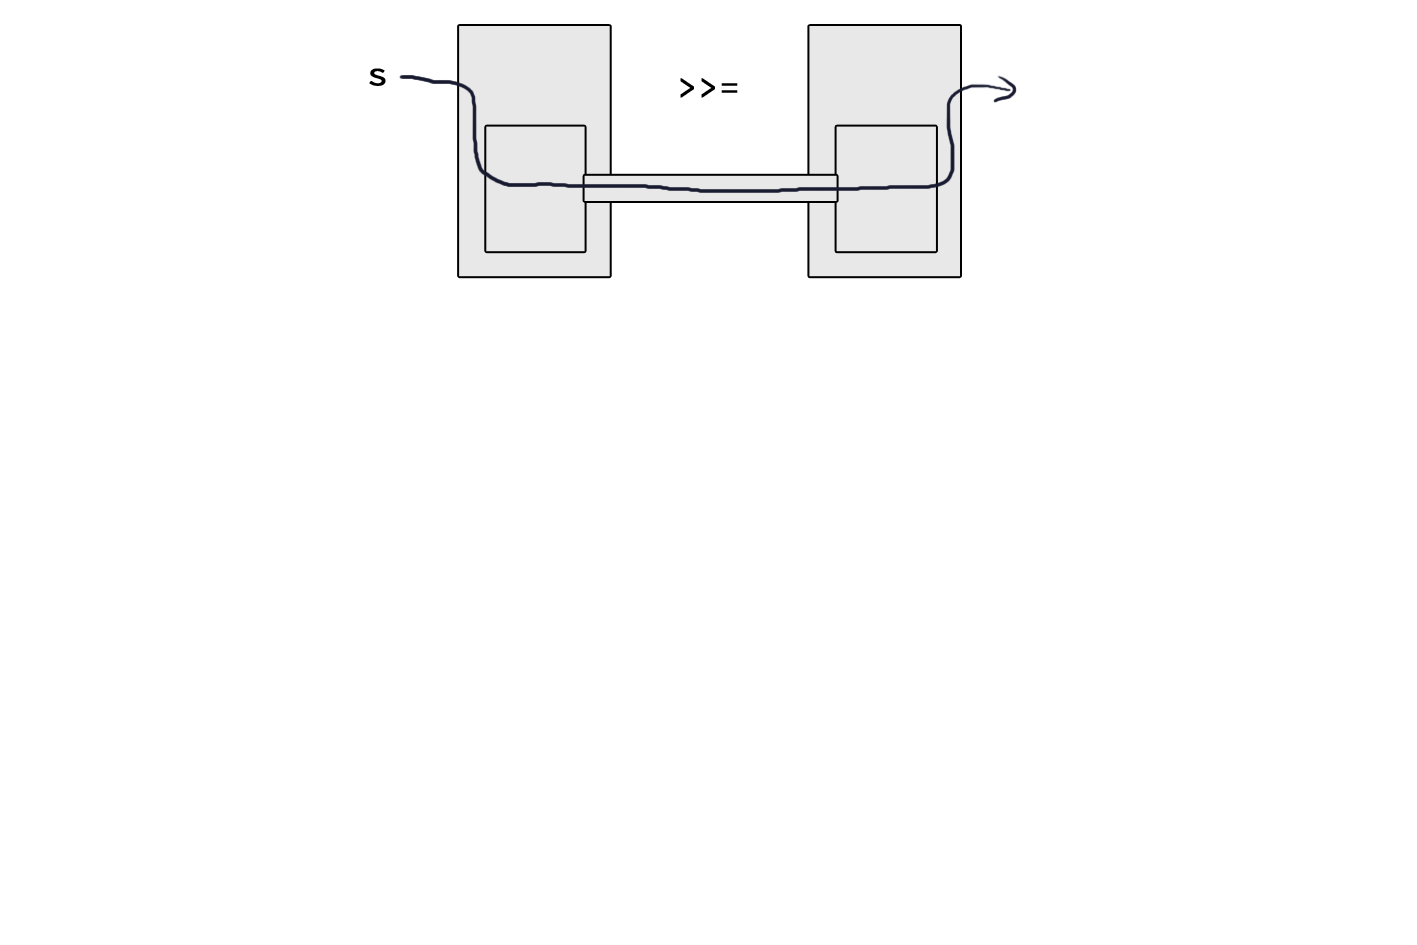
\includegraphics[width=\textwidth]{workfiles/v8_1}
		\end{figure}

	% subsection weltveraenderung (end)

	%%%
	%%% end V8
	%%%